\clearpage
\SourceLeaf{239}%
\begin{center}
{\Large\textsc{[Volumenbestimmungen\\ in der nichteuklidischen Geometrie.]}}



[1.]

\textsc{Gauss} an \textsc{Encke}. Göttingen, 1. Februar 1841.
\end{center}


\mbox{.\ .\ .\ .\ .\ .} Ich fange an, das Russische mit einiger Fertigkeit zu lesen, und
finde dabei viel Vergnügen. Hr. \textsc{Knorre} hat mir eine kleine in russischer
Sprache geschriebene Abhandlung von \textsc{Lobatschewsky} (in Kasan) geschickt und
dadurch so wie durch eine kleine Schrift in deutscher Sprache über Parallellinien
(wovon eine höchst alberne Anzeige in \textsc{Gersdorfs} Repertorium steht) bin ich
recht begierig geworden, mehr von diesem scharfsinnigen Mathematiker zu lesen. Wie mir
\textsc{Knorre} sagte, enthalten die (in russischer Sprache geschriebenen)
Abhandlungen der Universität Kasan eine Menge Aufsätze von ihm. \mbox{.\ .\ .}

\begin{center}


[2.]

\textsc{Astralgeometrie.}
\end{center}

\begin{center}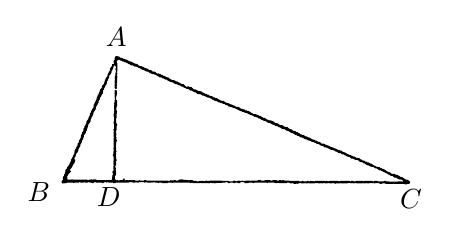
\begin{tikzpicture}[x=0.00534430cm,y=-0.00534430cm]
\fill[even odd rule] (99,387) -- (99,390) -- (101,392) -- (111,391) -- (112,390) -- (126,390) -- (128,391) -- (129,390) -- (140,390) -- (141,389) -- (143,389) -- (144,390) -- (151,390) -- (152,389) -- (154,389) -- (155,390) -- (161,390) -- (162,389) -- (165,389) -- (166,390) -- (171,390) -- (172,391) -- (174,391) -- (177,389) -- (180,389) -- (181,390) -- (195,390) -- (196,391) -- (198,391) -- (201,389) -- (205,389) -- (206,390) -- (208,389) -- (210,389) -- (211,390) -- (221,390) -- (222,391) -- (227,391) -- (228,390) -- (259,390) -- (260,389) -- (267,389) -- (268,390) -- (274,390) -- (275,389) -- (277,389) -- (278,390) -- (282,390) -- (283,389) -- (295,389) -- (296,390) -- (298,390) -- (299,389) -- (301,389) -- (302,390) -- (312,390) -- (314,389) -- (315,390) -- (317,390) -- (318,389) -- (320,389) -- (321,390) -- (328,390) -- (329,391) -- (331,390) -- (337,390) -- (338,391) -- (351,391) -- (352,390) -- (361,390) -- (362,391) -- (364,390) -- (404,390) -- (405,391) -- (410,390) -- (411,391) -- (427,391) -- (429,390) -- (430,391) -- (449,391) -- (450,392) -- (454,390) -- (456,391) -- (462,391) -- (464,392) -- (465,391) -- (488,390) -- (489,389) -- (493,389) -- (495,391) -- (499,391) -- (500,390) -- (507,390) -- (508,391) -- (511,391) -- (512,390) -- (517,390) -- (518,391) -- (523,391) -- (525,389) -- (533,389) -- (535,391) -- (543,391) -- (544,390) -- (553,390) -- (554,391) -- (556,391) -- (557,390) -- (587,390) -- (588,391) -- (590,390) -- (605,390) -- (606,391) -- (612,391) -- (614,390) -- (615,391) -- (634,391) -- (635,390) -- (640,390) -- (643,392) -- (649,391) -- (651,393) -- (656,393) -- (657,392) -- (661,393) -- (663,391) -- (668,391) -- (669,392) -- (676,392) -- (677,391) -- (679,391) -- (680,392) -- (684,392) -- (685,391) -- (687,391) -- (688,392) -- (701,392) -- (702,391) -- (709,391) -- (710,392) -- (714,392) -- (715,391) -- (717,391) -- (718,392) -- (720,392) -- (721,391) -- (725,391) -- (726,392) -- (736,391) -- (737,392) -- (742,392) -- (743,391) -- (746,391) -- (750,393) -- (751,392) -- (761,392) -- (762,391) -- (764,392) -- (778,392) -- (779,391) -- (783,391) -- (785,390) -- (787,392) -- (789,391) -- (792,391) -- (793,392) -- (795,392) -- (796,391) -- (801,391) -- (802,392) -- (814,392) -- (815,391) -- (817,391) -- (818,392) -- (820,392) -- (821,391) -- (823,392) -- (825,391) -- (827,392) -- (829,392) -- (830,391) -- (841,391) -- (842,392) -- (844,392) -- (845,391) -- (853,391) -- (857,393) -- (860,393) -- (861,392) -- (869,392) -- (870,393) -- (886,393) -- (888,392) -- (889,393) -- (914,393) -- (915,394) -- (920,394) -- (921,393) -- (925,393) -- (928,391) -- (928,388) -- (926,386) -- (921,383) -- (918,383) -- (909,377) -- (906,377) -- (902,374) -- (898,372) -- (893,371) -- (890,369) -- (884,369) -- (879,365) -- (874,364) -- (869,360) -- (865,358) -- (863,358) -- (861,356) -- (857,355) -- (855,353) -- (851,353) -- (850,352) -- (848,352) -- (840,348) -- (836,345) -- (834,345) -- (829,342) -- (826,342) -- (824,340) -- (821,340) -- (819,338) -- (814,337) -- (812,335) -- (810,335) -- (807,332) -- (805,332) -- (804,331) -- (800,331) -- (796,328) -- (793,328) -- (790,326) -- (788,326) -- (786,324) -- (783,324) -- (772,318) -- (768,317) -- (765,314) -- (762,314) -- (761,313) -- (756,312) -- (751,309) -- (749,309) -- (746,307) -- (739,305) -- (734,302) -- (732,302) -- (730,300) -- (727,300) -- (722,297) -- (717,297) -- (714,294) -- (712,293) -- (709,293) -- (706,290) -- (702,290) -- (700,288) -- (695,287) -- (689,283) -- (687,283) -- (681,280) -- (679,280) -- (675,277) -- (672,277) -- (669,275) -- (667,275) -- (664,272) -- (662,272) -- (660,270) -- (658,270) -- (654,267) -- (650,267) -- (645,263) -- (643,263) -- (639,261) -- (636,258) -- (629,257) -- (623,253) -- (618,253) -- (613,249) -- (607,248) -- (602,244) -- (600,244) -- (597,242) -- (593,242) -- (592,241) -- (590,241) -- (586,239) -- (583,236) -- (579,236) -- (571,231) -- (569,231) -- (566,229) -- (563,229) -- (561,227) -- (555,227) -- (552,224) -- (550,224) -- (548,222) -- (544,220) -- (542,220) -- (539,218) -- (536,218) -- (534,216) -- (531,216) -- (530,215) -- (525,214) -- (520,210) -- (514,210) -- (511,207) -- (509,207) -- (503,204) -- (501,204) -- (495,201) -- (493,201) -- (487,198) -- (485,196) -- (478,195) -- (468,189) -- (465,189) -- (463,187) -- (460,187) -- (458,185) -- (450,183) -- (448,181) -- (446,181) -- (443,179) -- (440,179) -- (438,177) -- (433,175) -- (431,173) -- (424,172) -- (416,168) -- (413,168) -- (408,163) -- (402,162) -- (401,161) -- (395,162) -- (389,156) -- (383,155) -- (381,153) -- (376,151) -- (374,149) -- (371,149) -- (366,146) -- (362,146) -- (356,143) -- (353,140) -- (347,139) -- (345,137) -- (341,136) -- (339,134) -- (337,134) -- (334,132) -- (332,132) -- (330,130) -- (326,131) -- (321,126) -- (316,126) -- (313,123) -- (307,122) -- (303,119) -- (296,117) -- (294,115) -- (292,115) -- (289,113) -- (286,113) -- (282,111) -- (279,108) -- (273,107) -- (266,103) -- (259,101) -- (255,98) -- (247,96) -- (244,94) -- (239,93) -- (235,90) -- (232,90) -- (231,89) -- (228,89) -- (225,94) -- (225,98) -- (223,100) -- (223,104) -- (224,106) -- (222,108) -- (220,108) -- (219,109) -- (219,112) -- (214,119) -- (214,124) -- (211,127) -- (211,129) -- (209,131) -- (208,137) -- (204,142) -- (204,144) -- (202,146) -- (202,149) -- (201,150) -- (200,155) -- (196,159) -- (195,161) -- (195,164) -- (191,168) -- (189,175) -- (187,177) -- (187,180) -- (185,182) -- (185,184) -- (183,187) -- (182,192) -- (175,206) -- (175,211) -- (172,215) -- (171,218) -- (169,220) -- (169,223) -- (167,225) -- (167,228) -- (163,236) -- (163,238) -- (158,245) -- (158,249) -- (156,251) -- (156,253) -- (153,257) -- (153,260) -- (151,262) -- (151,267) -- (147,271) -- (147,274) -- (145,278) -- (145,282) -- (142,288) -- (140,290) -- (141,293) -- (138,296) -- (137,298) -- (137,301) -- (130,314) -- (129,322) -- (126,326) -- (126,328) -- (122,335) -- (122,337) -- (116,349) -- (112,354) -- (112,356) -- (108,360) -- (108,365) -- (107,366) -- (107,369) -- (105,371) -- (105,374) -- (102,377) -- (102,380) -- (103,382) -- cycle
(112,375) -- (114,373) -- (116,369) -- (121,364) -- (121,363) -- (119,361) -- (119,359) -- (124,353) -- (126,348) -- (130,343) -- (130,341) -- (131,340) -- (131,336) -- (129,332) -- (132,328) -- (134,321) -- (137,318) -- (139,314) -- (139,311) -- (144,302) -- (144,299) -- (147,294) -- (147,291) -- (150,287) -- (150,285) -- (152,281) -- (152,278) -- (157,271) -- (157,268) -- (159,266) -- (159,263) -- (160,262) -- (163,251) -- (166,248) -- (168,244) -- (168,240) -- (170,237) -- (170,235) -- (172,233) -- (172,231) -- (174,229) -- (175,223) -- (180,216) -- (181,210) -- (183,206) -- (185,204) -- (185,202) -- (187,200) -- (187,196) -- (190,192) -- (190,188) -- (193,185) -- (195,180) -- (197,178) -- (198,170) -- (200,168) -- (200,165) -- (202,163) -- (204,158) -- (206,156) -- (206,154) -- (207,153) -- (207,149) -- (209,147) -- (209,145) -- (211,143) -- (211,141) -- (212,140) -- (212,136) -- (215,133) -- (218,127) -- (218,125) -- (221,120) -- (223,113) -- (225,111) -- (226,111) -- (229,116) -- (229,117) -- (227,119) -- (227,121) -- (228,122) -- (228,128) -- (227,129) -- (227,135) -- (226,136) -- (226,140) -- (225,141) -- (226,143) -- (226,147) -- (225,148) -- (225,153) -- (226,154) -- (226,156) -- (225,157) -- (225,165) -- (227,167) -- (229,167) -- (231,165) -- (230,163) -- (230,161) -- (231,160) -- (230,155) -- (231,154) -- (231,141) -- (232,140) -- (232,138) -- (231,137) -- (231,132) -- (232,131) -- (231,129) -- (231,125) -- (232,124) -- (232,107) -- (230,104) -- (230,102) -- (233,98) -- (237,98) -- (239,100) -- (241,100) -- (244,102) -- (247,102) -- (249,104) -- (252,104) -- (256,106) -- (258,108) -- (260,108) -- (264,111) -- (268,111) -- (273,114) -- (277,114) -- (278,115) -- (280,115) -- (283,118) -- (285,118) -- (292,122) -- (294,122) -- (302,126) -- (305,126) -- (307,128) -- (315,132) -- (319,132) -- (320,133) -- (322,133) -- (333,140) -- (337,140) -- (339,142) -- (341,142) -- (346,145) -- (349,145) -- (351,147) -- (357,150) -- (364,152) -- (370,156) -- (373,156) -- (379,159) -- (381,159) -- (385,162) -- (387,162) -- (392,165) -- (394,165) -- (396,167) -- (399,167) -- (403,169) -- (405,171) -- (409,171) -- (411,173) -- (419,176) -- (422,179) -- (430,180) -- (434,183) -- (437,183) -- (447,188) -- (450,188) -- (456,191) -- (458,193) -- (460,193) -- (462,195) -- (468,196) -- (472,199) -- (475,199) -- (478,201) -- (481,201) -- (483,203) -- (487,203) -- (490,206) -- (493,206) -- (496,209) -- (499,209) -- (500,210) -- (505,211) -- (508,213) -- (511,213) -- (525,220) -- (527,220) -- (529,222) -- (532,222) -- (533,223) -- (541,225) -- (543,227) -- (545,227) -- (547,229) -- (550,229) -- (556,232) -- (558,234) -- (561,233) -- (563,235) -- (565,235) -- (568,238) -- (571,238) -- (575,241) -- (577,241) -- (580,243) -- (582,243) -- (588,246) -- (590,248) -- (594,248) -- (601,252) -- (605,253) -- (607,255) -- (613,256) -- (615,258) -- (619,259) -- (623,262) -- (630,263) -- (633,266) -- (638,267) -- (642,270) -- (646,272) -- (648,272) -- (656,277) -- (658,277) -- (660,279) -- (663,279) -- (667,282) -- (672,283) -- (679,287) -- (681,287) -- (687,290) -- (692,291) -- (694,293) -- (698,293) -- (700,295) -- (704,296) -- (706,298) -- (710,298) -- (716,302) -- (721,303) -- (724,306) -- (728,306) -- (740,312) -- (744,312) -- (747,314) -- (749,314) -- (751,316) -- (753,316) -- (757,319) -- (763,320) -- (766,323) -- (770,323) -- (772,325) -- (774,325) -- (778,328) -- (784,329) -- (788,333) -- (792,333) -- (798,336) -- (803,336) -- (809,341) -- (814,341) -- (817,344) -- (820,344) -- (823,347) -- (827,349) -- (829,349) -- (834,352) -- (841,353) -- (845,356) -- (848,356) -- (855,361) -- (858,361) -- (874,369) -- (876,371) -- (878,371) -- (882,374) -- (886,374) -- (890,378) -- (895,378) -- (897,380) -- (901,382) -- (903,382) -- (904,383) -- (908,383) -- (911,385) -- (911,387) -- (910,388) -- (908,387) -- (879,388) -- (878,387) -- (871,387) -- (870,386) -- (866,386) -- (865,387) -- (851,387) -- (850,386) -- (843,386) -- (842,387) -- (839,387) -- (838,386) -- (819,386) -- (818,387) -- (816,386) -- (799,386) -- (798,387) -- (794,387) -- (793,386) -- (788,386) -- (787,387) -- (785,387) -- (784,386) -- (761,386) -- (760,387) -- (758,387) -- (757,386) -- (735,386) -- (734,387) -- (732,387) -- (731,386) -- (728,386) -- (727,387) -- (725,386) -- (702,386) -- (701,387) -- (690,386) -- (689,387) -- (687,387) -- (686,386) -- (683,386) -- (682,387) -- (674,387) -- (673,386) -- (671,386) -- (670,387) -- (665,387) -- (664,386) -- (641,386) -- (640,385) -- (629,385) -- (628,384) -- (626,385) -- (624,384) -- (622,385) -- (620,384) -- (617,384) -- (616,385) -- (611,385) -- (610,384) -- (601,384) -- (600,385) -- (596,385) -- (595,384) -- (583,384) -- (582,385) -- (573,385) -- (572,384) -- (566,384) -- (565,385) -- (550,385) -- (549,386) -- (547,386) -- (546,385) -- (537,385) -- (536,386) -- (530,386) -- (529,385) -- (527,386) -- (523,386) -- (522,385) -- (519,385) -- (516,387) -- (512,386) -- (511,385) -- (507,386) -- (506,387) -- (497,387) -- (496,386) -- (480,386) -- (479,385) -- (452,385) -- (451,386) -- (445,386) -- (444,385) -- (442,385) -- (438,387) -- (436,386) -- (426,386) -- (425,387) -- (421,387) -- (420,386) -- (413,386) -- (410,384) -- (404,384) -- (402,385) -- (401,384) -- (387,383) -- (386,382) -- (379,383) -- (376,385) -- (371,385) -- (370,384) -- (360,385) -- (358,384) -- (356,386) -- (352,386) -- (351,385) -- (346,385) -- (345,386) -- (343,385) -- (332,385) -- (331,386) -- (329,385) -- (301,385) -- (300,384) -- (296,384) -- (295,385) -- (286,385) -- (285,384) -- (283,385) -- (274,385) -- (273,384) -- (268,384) -- (267,385) -- (265,384) -- (260,384) -- (258,385) -- (257,384) -- (252,384) -- (251,385) -- (249,383) -- (249,381) -- (248,380) -- (247,380) -- (244,384) -- (238,384) -- (237,385) -- (231,384) -- (229,385) -- (226,381) -- (226,375) -- (229,370) -- (229,364) -- (228,363) -- (228,360) -- (227,359) -- (228,357) -- (228,355) -- (227,354) -- (227,350) -- (229,348) -- (229,344) -- (228,343) -- (229,342) -- (229,339) -- (230,338) -- (230,335) -- (229,334) -- (229,329) -- (228,328) -- (228,325) -- (229,324) -- (229,317) -- (230,316) -- (228,312) -- (229,310) -- (228,304) -- (229,303) -- (229,294) -- (231,289) -- (229,287) -- (229,285) -- (230,284) -- (229,282) -- (229,276) -- (230,275) -- (229,274) -- (229,266) -- (230,265) -- (230,255) -- (231,254) -- (231,251) -- (229,248) -- (229,240) -- (228,239) -- (228,238) -- (230,236) -- (230,229) -- (229,227) -- (231,225) -- (230,223) -- (231,220) -- (229,217) -- (230,209) -- (231,208) -- (231,195) -- (229,193) -- (229,185) -- (230,184) -- (230,181) -- (231,180) -- (230,170) -- (226,170) -- (225,171) -- (225,187) -- (226,188) -- (226,193) -- (225,194) -- (225,199) -- (224,200) -- (224,202) -- (225,203) -- (224,205) -- (224,216) -- (225,218) -- (224,219) -- (224,225) -- (223,226) -- (223,233) -- (224,234) -- (224,244) -- (223,245) -- (223,251) -- (224,252) -- (224,262) -- (222,264) -- (222,265) -- (224,267) -- (223,269) -- (223,281) -- (224,283) -- (223,284) -- (223,308) -- (222,309) -- (223,311) -- (223,315) -- (222,316) -- (222,322) -- (221,323) -- (221,325) -- (223,329) -- (223,338) -- (222,339) -- (222,341) -- (223,342) -- (222,344) -- (222,346) -- (223,347) -- (223,350) -- (222,351) -- (222,357) -- (223,358) -- (223,360) -- (220,364) -- (220,366) -- (221,367) -- (221,371) -- (220,372) -- (220,376) -- (219,377) -- (219,382) -- (217,384) -- (205,384) -- (204,385) -- (202,384) -- (183,384) -- (180,382) -- (174,382) -- (173,383) -- (169,382) -- (168,383) -- (164,383) -- (163,384) -- (161,384) -- (160,383) -- (126,383) -- (125,382) -- (123,382) -- (122,383) -- (114,383) -- (113,382) -- (113,378) -- (112,377) -- cycle;
\node[inner sep=0pt] at (229,44) {$A$};
\node[inner sep=0pt] at (45,412) {$B$};
\node[inner sep=0pt] at (211,424) {$D$};
\node[inner sep=0pt] at (930,430) {$C$};
\end{tikzpicture}
\end{center}


$Aa$, $Bb$, $Cc$ normal gegen die Ebene, worin das Dreieck $ABC$. Durch $a$, $b$, $c$
eine zweite Ebene.


$Aa$ kleinster Abstand der beiden Ebenen, und selbst unendlich klein. $AD$ normal
gegen $BC$.
